% --------------------------------------
% Document Class
% --------------------------------------
\documentclass[a4paper,11pt]{article}
% --------------------------------------



% --------------------------------------
% Use Package
% --------------------------------------


\usepackage[francais]{babel}
%\usepackage{ucs}
\usepackage[utf8]{inputenc}
\usepackage[T1]{fontenc}

\usepackage{makeidx}
\usepackage{color}
\usepackage{graphicx}
\usepackage{float}
\usepackage[hidelinks]{hyperref} 
\usepackage{geometry}
%\usepackage{lastpage}
%\usepackage{marginnote}
\usepackage{fancyhdr}
%\usepackage{titlesec}
%\usepackage{framed}
\usepackage{amsmath}
\usepackage{empheq}
\usepackage{array}
\usepackage{multicol}
\usepackage{csquotes}
%\usepackage{adjustbox}

% insert code
\usepackage{listings}

% define our color
\usepackage{xcolor}

% code color
\definecolor{ligthyellow}{RGB}{250,247,220}
\definecolor{darkblue}{RGB}{5,10,85}
\definecolor{ligthblue}{RGB}{1,147,128}
\definecolor{darkgreen}{RGB}{8,120,51}
\definecolor{darkred}{RGB}{160,0,0}

% other color
\definecolor{ivi}{RGB}{141,107,185}


\lstset{
    language=Scilab,
    captionpos=b,
    extendedchars=true,
    frame=lines,
    numbers=left,
    numberstyle=\tiny,
    numbersep=5pt,
    keepspaces=true,
    breaklines=true,
    showspaces=false,
    showstringspaces=false,
    breakatwhitespace=false,
    stepnumber=1,
    showtabs=false,
    tabsize=3,
    basicstyle=\small\ttfamily,
    backgroundcolor=\color{ligthyellow},
    keywordstyle=\color{ligthblue},
    morekeywords={include, printf, uchar},
    identifierstyle=\color{darkblue},
    commentstyle=\color{darkgreen},
    stringstyle=\color{darkred},
}


% --------------------------------------



% --------------------------------------
% Page setting
% --------------------------------------
%\pagestyle{empty}
\setlength{\headheight}{15pt}

\setcounter{secnumdepth}{3}
\setcounter{tocdepth}{2}

\makeatletter
\@addtoreset{chapter}{part}
\makeatother 

\hypersetup{         % parametrage des hyperliens
  colorlinks=true,      % colorise les liens
  breaklinks=true,      % permet les retours à la ligne pour les liens trop longs
  urlcolor= blue,       % couleur des hyperliens
  linkcolor= black,     % couleur des liens internes aux documents (index, figures, tableaux, equations,...)
  citecolor= green      % couleur des liens vers les references bibliographiques
}

% --------------------------------------

% --------------------------------------
% Information
% --------------------------------------
\title{Compte-rendu TP7 TI : Atténuation du phénomène de Moiré}
\author{Elliot VANEGUE et Gaëtan DEFLANDRE}
% --------------------------------------

\definecolor{myColor}{rgb}{0.5, 0.1, 0.75}

% --------------------------------------
% Begin content
% --------------------------------------
\begin{document}

% Set language to english
  \selectlanguage{francais}

  % Start the page counting
  \pagenumbering{arabic}

  \maketitle
  
  \mbox{}
  \newpage
  \clearpage
  
  \section*{Introduction}
  Pour certaines répétitions de motifs dans une image, nous pouvons observer un phénomène qui déforme ce motif, selon différentes conditions. 
  Ce phénomène est appelé le phénomène de Moiré. Il se produit lorsque la fréquence d’un motif est trop grande. Le but de ce TP va être de 
  comprendre et de trouver une solution pour éviter ce phénomène quelque soit l’image.\\
 
  \section{Étude des fréquences}
  Pour l’étude du phénomène de moiré, nous disposons de trois images (cf Figure 1). L’image \textit{1024\_moire\_f1} avec une grande fréquence, 
  l’image \textit{1024\_moire\_f2} avec une une fréquence inférieure à l’image $f1$ et l’image \textit{1024\_moire} qui est l’addition des images 
  $f1$ et $f2$. Nous pouvons obtenir l’image \textit{1024\_moire} dans le menu Process $\rightarrow$ Image Calculator\ldots grâce à l’opération 
  \textbf{Add} sur l’image $f1$ et $f2$.\\

  \begin{figure}[H]
   \centering
   \shortstack{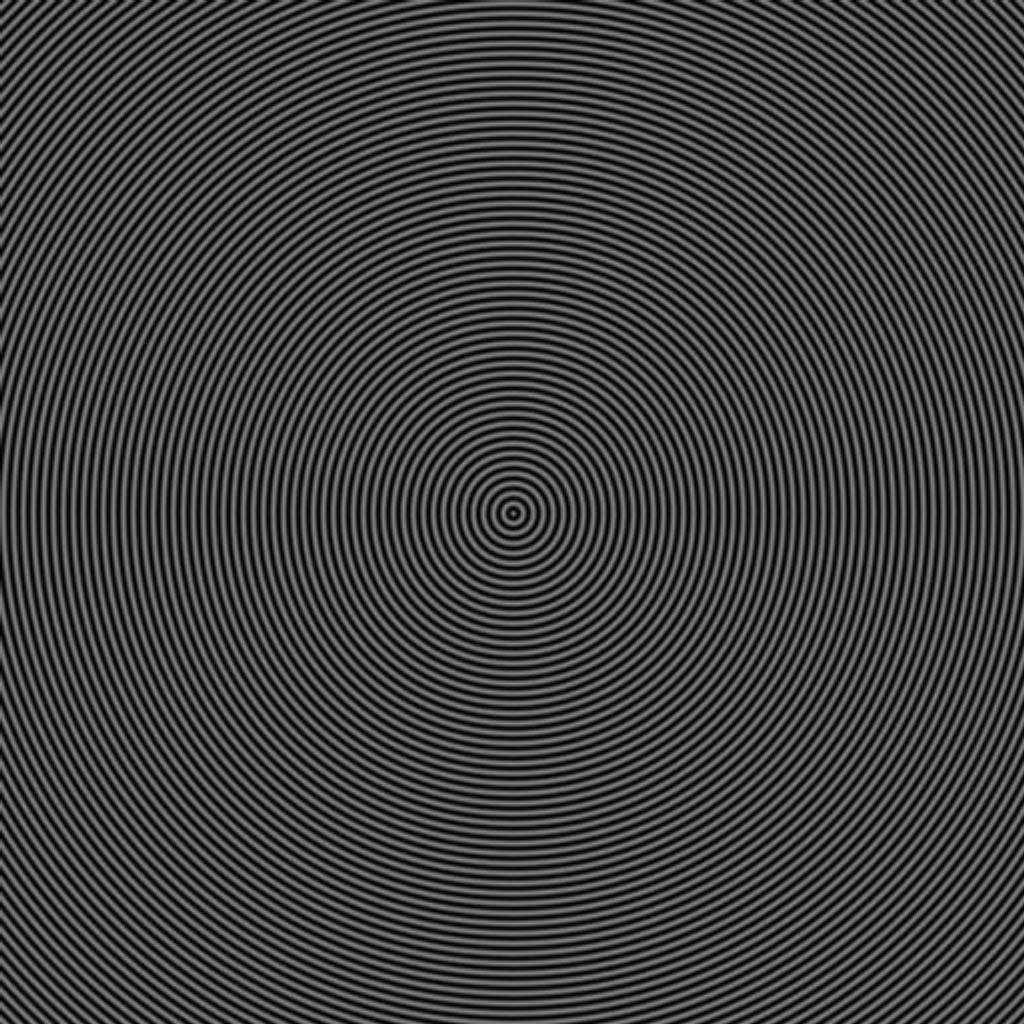
\includegraphics[width=4.5cm]{../1024_moire_f1.png} \\ {\small1024\_moire\_f1.png}}
   \shortstack{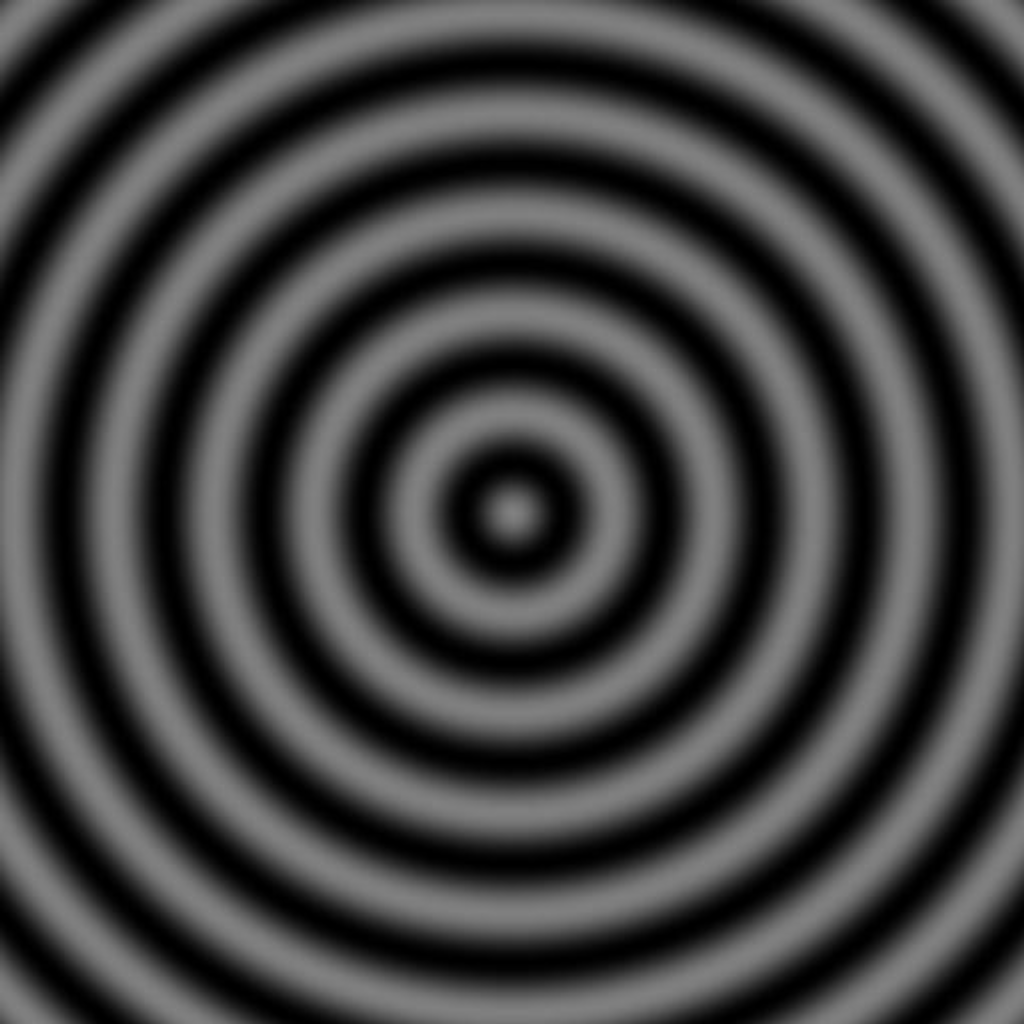
\includegraphics[width=4.5cm]{../1024_moire_f2.png} \\ {\small1024\_moire\_f2.png}}
   \shortstack{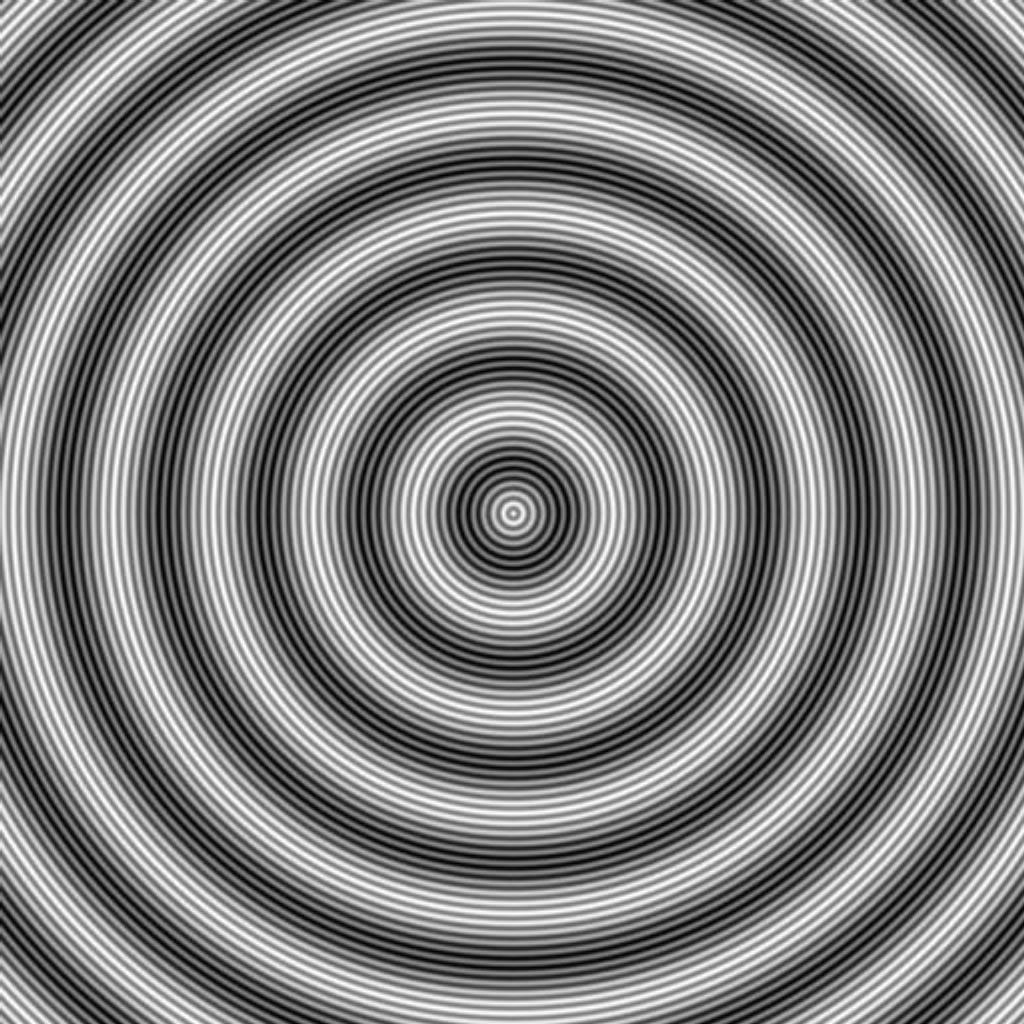
\includegraphics[width=4.5cm]{../1024_moire.png} \\ {\small1024\_moire.png}}
   \caption{Images présentes pour le TP}
  \end{figure}

  La période spatiale de l’image $f1$ est de 10 pixels, ce qui donne une fréquence de $\frac{1}{10}$. Pour l’image $f2$, la période est de 100 pixels, 
  donc la fréquence est de $\frac{1}{100}$. Nous pouvons retrouver les fréquences de ces images dans le plan de Fourier, c’est la taille du rayon du cercle 
  qui a pour centre le centre du plan de Fourier. Nous remarquons également que la transformée de l’image \textit{1024\_moire} correspond aux maximums  
  des transformées de Fourier des images $f1$ et $f2$, que nous pouvons obtenir grâce à l’opérateur \textbf{Max} du menu Process $\rightarrow$ Image Calculator, 
  sur les transformées de $f1$ et $f2$.\\
  
  \section{Théorème de Shannon}
  Le théorème de Shannon nous dit que : \enquote{La représentation discrète d'un signal par des échantillons régulièrement espacés exige une fréquence d'échantillonnage 
  supérieure au double de la fréquence maximale présente dans ce signal.}. Lorsque nous réduisons la taille de l’image et que nous la divisons par deux, les fréquences 
  présentes dans l’image sont multipliées par deux, car le nombre de pixels entre deux motifs est divisé par deux. L’image résultante au changement d’échelle n’a aucun effet 
  de Moiré visible sur l’image. Donc l’échantillonage respecte le théorème de Shannon.\\
  
  En revanche, quand nous effectuons un échantillonage d’un facteur 1/8\up{ème}, nous pouvons observer une légère déformation des motifs de l’image. Cela s’accentue 
  d’avantage en diminuant la taille de l’image. Donc à partir d’un certain seuil, le théorème de Shannon n’est plus respecté. 
  Si on a $2*f_1=\frac{1}{10}$ alors la fréquence d'échantillonage maximum est $\frac{1}{5}$, car par la suite nous aurons $2*f_1$ < <fréquence échantillonage>.\\
% Si on a $f_1=\frac{1}{10}$ alors la fréquence d'échantillonage maximum est $2*f1$, soit $\frac{1}{5}$, car par la suite nous aurons $2*f_1$ < <fréquence échantillonage>.\\
  
  \begin{figure}[H]
   \centering
   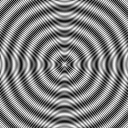
\includegraphics[width=4cm]{../128_moire.png}
   \caption{Effet de Moiré}
  \end{figure}


  On voit que parmi les deux fréquences présentes dans l’image, seule la fréquence la plus grande subit l’effet de Moiré. Cela paraît logique avec le thèorème de Shannon, 
  puisqu’il y a une seule fréquence d’échantillonage et deux fréquences dans l’image, donc ce sera toujours la fréquence la plus grande qui subira, en premier, l’effet de Moiré.\\

  Le repliement de spectre est un phénomène qui introduit des fréquences inexistantes dans un signal, dans notre cas cela se produit lorsque le théorème de Shannon n’est pas respecté.
  Le problème survient lorsque la fréquence maximale d’un motif est atteinte, soit $\frac{1}{2}$.\\

  \section{Solution au phénomène de Moiré}
  
  Pour remédier au phénomène de Moiré, nous avons atténué les basses fréquences de l'image. C'est à dire qu'on a pris un
  seuil sur les descripteurs de Fourier et qu'au delà de ce seuil, nous avons supprimé toutes les fréquences. Dans une image,
  ce procédé va la flouter. Dans notre cas, les plus petites rayures, donc celles dont la fréquence est la plus grande,
  vont être supprimées. Ainsi lorsque nous allons changer la fréquence d'échantillonage de l'image, nous n'aurons plus de phénomènes
  de Moiré puisque ce phénomène était lié aux plus hautes fréquences.\\
  
  \begin{figure}[H]
  \center
   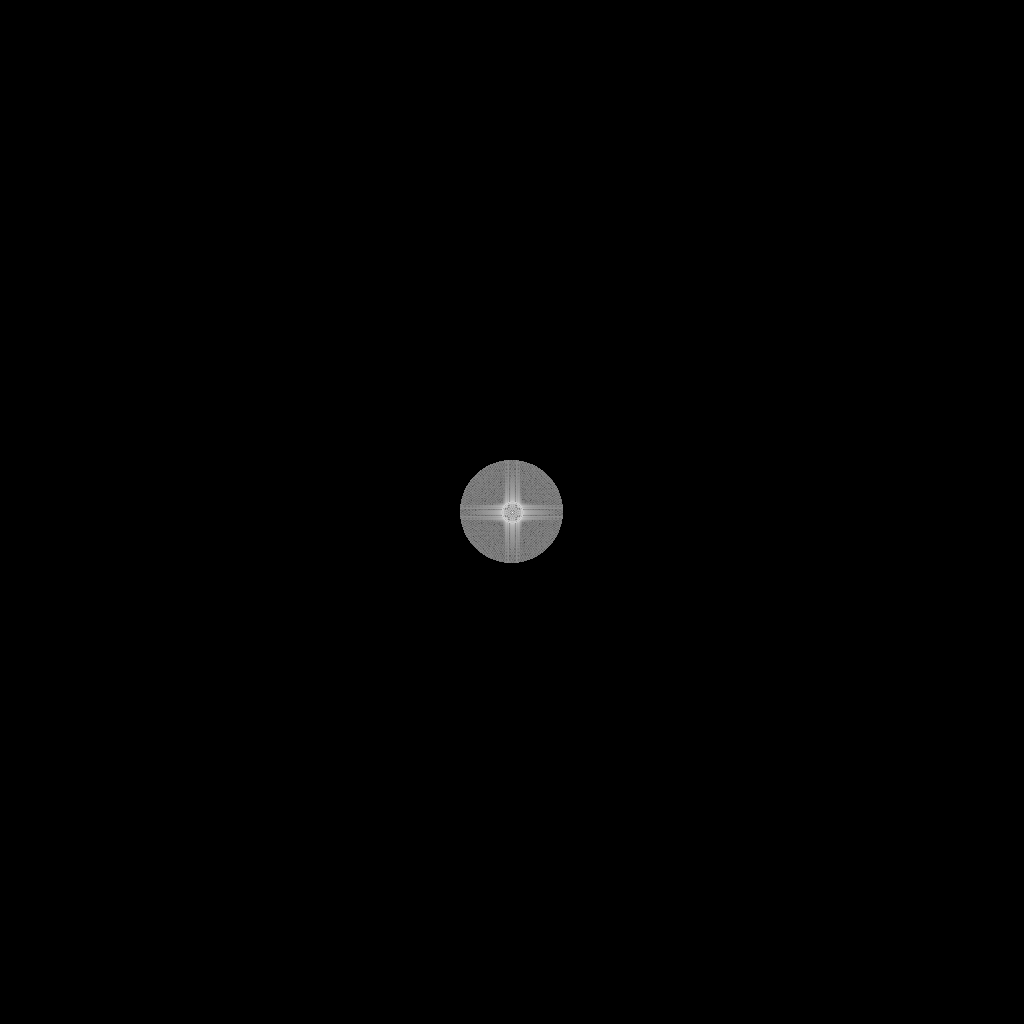
\includegraphics[width=5cm]{../FFT_1024_moire.png}
   \caption{Transformée de Fourier avec filtre passe-bas}
  \end{figure}
  
  Pour ce cas d'étude, nous avons pris un seuil de 0.05, car ce seuil se trouve entre les deux fréquences de l'image et donc 
  élimine seulement la plus grande.
  
  \begin{figure}[H]
  \center
   
\includegraphics[width=5cm]{../1024_moire_hf.png}
   \caption{Résultat du filtre passe-bas}
  \end{figure}
  
  \section{Conclusion}
  Durant ce TP, nous avons vu que les fréquences dans une image peuvent jouer un rôle important. Elles peuvent
  accentuer le bruit de l'image et provoquer des repliements de spectre. Les filtres passe-bas peuvent s'avérer
  particulièrement utiles dans ce genre de situation. Il peuvent permettre d'atténuer du bruit, mais cela peut
  provoquer une perte d'information non négligeable sur un signal.
  
  \newpage
  \section{Annexes}
  \begin{lstlisting}[caption=Macro d'atténuation du phénomène de Moiré]
macro "filtrage passe-basFFT" {

    run("FFT");
    // recuperation de ID de la FFT
    fourier = getImageID();

    // recuperation de la taille W x H du plan de Fourier
    W = getWidth();
    H = getHeight();

    // Creation d'un masque binaire
    newImage("masque", "8-bit", W, H, 1);
    masque = getImageID();
    // fond noir
    setColor(0);
    makeRectangle (0,0, W,H);
    fill();

    fc = 0.05;

    // calcul du rayon du disque binaire à partir de la frequence de coupure fc
    // attention, la FFT etant consideree comme une image par ImageJ, le rayon doit etre calcule en pixels
    rayon = H * fc;
    print("rayon =", rayon);

    setColor(255);
    makeOval (W/2-rayon,H/2-rayon, 2*rayon,2*rayon);
    fill ();


    // Filtrage passe-bas
    selectImage(fourier);
    makeOval(W/2-rayon,H/2-rayon, 2*rayon,2*rayon);
    setColor(0);
    // Selection inverse du cercle
    run("Make Inverse");
    fill();

    // Transformee de fourier inverse pour fournir l'image filtree
    run("Inverse FFT");
}
  \end{lstlisting}


\end{document}  